\subsection{DTW Alignment as an Adaptive Resampling Strategy}

In this section, we present a method that uses Dynamic Time Warping (DTW)
on multimodal time series, \emph{i.e.} time series that are made of several
features recorded over time.
The method relies on the assumption that one of the considered modalities
(called
reference modality in the following) can be used as a reference to (temporally)
realign other modalities~\cite{dupas:halshs-01228397}.
It has been used in the context of hydrological measurements to align pollutant
concentration profiles based on discharge time series.%
\footnote{This work is a part of Rémi Dupas' PhD thesis (in Environment
Sciences).
I was not directly involved in the supervision of Rémi's PhD thesis.}

This approach can be seen as the DTW counterpart of other works that rely on
Optimal Transport for Domain Adaptation~\cite{courty:hal-02112785}.
One significant difference, however, is that it relies on a reference modality
for
alignment.
This design choice is guided by our application context.

\subsubsection{Motivating Use Case}

Phosphorus (P) transfer during storm events represents a significant part of
annual P loads in streams and contributes to eutrophication in downstream water
bodies. To improve understanding of P storm dynamics, automated or
semi-automated methods are needed to extract meaningful information from
ever-growing water quality measurement datasets.

Clustering techniques have proven useful for identifying seasonal storm
patterns and thus for increasing knowledge about seasonal variability in storm
export mechanisms (\emph{e.g.},~\cite{aubert:halshs-00906292}).
Clustering techniques usually require calculating distances between pairs of
comparable points in multiple time series. For this reason, direct clustering
(without using hysteresis-descriptor variables) of high-frequency storm
concentration time series is usually irrelevant because the lengths of recorded
time series (number of
measurement points) might differ and/or measurement points may have different
positions relative to the hydrograph (flow rise and recession); hence, it is
difficult to calculate a distance between pairs of comparable points.

The aim of this study was to develop a clustering method that overcomes this
limit and test its ability to compare seasonal variability of P storm dynamics
in two headwater watersheds. Both watersheds are ca. 5 km$^2$, have similar
climate and geology, but differ in land use and P pressure intensity.

\subsubsection{Alignment-based Resampling Method}

In the above-described setting, we have access to one modality (discharge,
commonly denoted $Q$) that is representative of the evolution of the flood.
Temporal realignment based on this modality allows to overcome three
difficulties that can arise when comparing storm-event data.
Indeed, time series can have

\begin{enumerate}
\item different starting times due to the discharge threshold at which the
samplers were triggered,
\item different lengths, and
\item differences in phase that yield different temporal localizations of the
discharge peak.
\end{enumerate}

To align time series, we use the path associated with DTW.
This matching path can be viewed as the optimal way to perform point-wise
alignment of time series.

For each discharge time series $\mathbf{x}^{(i)}_\text{Q}$, we compute the
matching path $\pi_\text{Q}$ and use it to find the optimal alignment wrt.
the same reference discharge time series $\mathbf{x}^\text{ref}_\text{Q}$.
The reference discharge time series used in this study is chosen
as a storm event with full coverage of flow rise and flow recession phases.
Alternatively, one could choose a synthetic idealized storm hydrograph.

We then use barycentric mapping based on the obtained matches to realign other
modalities to the timestamps of the reference time series, as shown in
Figure~\ref{fig:dtw_da}.

\begin{figure}[t]
    \begin{subfigure}[b]{\textwidth}
         \centering
         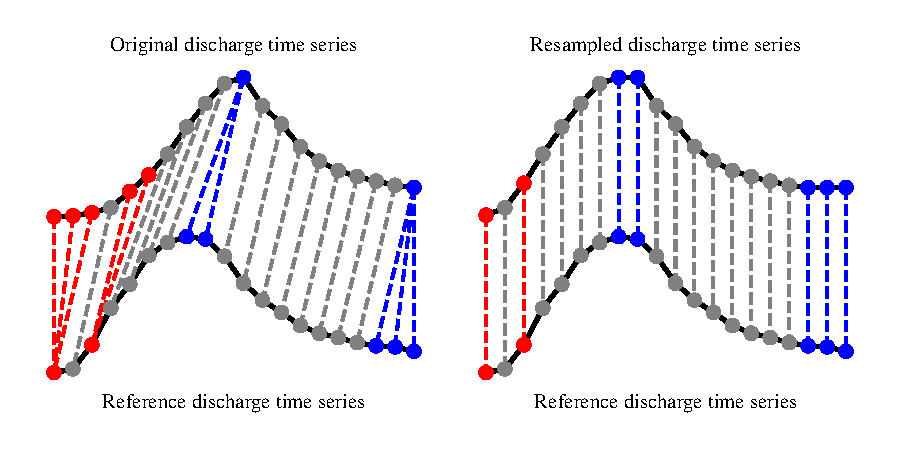
\includegraphics[width=.7\textwidth]{fig/dtw_da}
     \end{subfigure}
      \begin{subfigure}[b]{\textwidth}
           \centering
           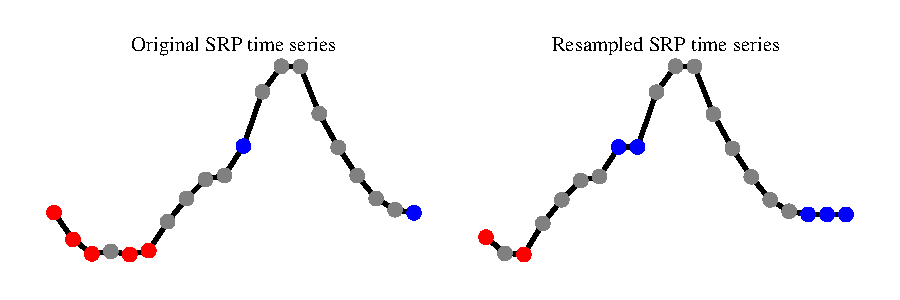
\includegraphics[width=.7\textwidth]{fig/dtw_da_b}
       \end{subfigure}
    \caption{Adaptive resampling strategy. Top row: A discharge time series is
    resampled so that its timestamps match those of a reference one. Bottom row:
    The same temporal transformation is applied to all other modalities
    (\emph{e.g.} SRP concentration) of the given sample.}
    \label{fig:dtw_da}
\end{figure}

At this point, each time series is transformed to series of $n$
$p$-dimensional measurements, where $n$ is the length of the
reference discharge time series and $p$ is the number of water quality
parameters considered in the study (\emph{i.e.} all modalities except the
discharge).
In a second step, a standard $k$-means algorithm is used to cluster
realigned time series.
Note that a Euclidean distance can be used for clustering since time series
have already been temporally realigned; hence, time-sensitive metrics (such as
DTW) are no longer needed.

This method proved useful to extract meaningful clusters and an \emph{a posteriori}
analysis of the clusters enabled to identify the export dynamics of pollutants
in different geographical areas of the study sites, which then led to management
recommendations, as detailed in~\cite{dupas:halshs-01228397}.
